\section{Requirements analysis}
There is a need to integrate external memory access into the \graicore{}'s architecture.
The addition of the external memory extends the total memory of system, allowing the system to store larger and multiple AI models.
The access to the external memory must be efficient in terms of throughput and power.
The external memory, along with the \graicore{}’s architecture, must provide a sufficiently high data transfer rate to load the \graicore{} with a new (partial) AI model seamlessly.

We consider two separate cases:
\begin{itemize}
    \item \textbf{Multiple models}: here we assume that the AI models are all exactly the size of the memory capacity of the \graicore{}.
    This implies that the complete memory of the \graicore{} must be written to load a new AI model.
    \item \textbf{Large model}: a large AI model is too large to be fitted onto the \graicore{}'s memory at once.
    Therefore, a large AI model must be run in parts by partitioning the model into smaller pieces.
\end{itemize}

\subsubsection{Multiple models}
The \graicore{} is unable to make use of multiple models as they do not fit in the local memories simultaneously.
Additionally, the \graicore{} lacks the ability to reconfigure itself during run-time.
The time it takes to process a frame is dependent on the complexity of the model on the \graicore{}.
Based on realistic use-cases with models executed on the \graicore{}, it has been established by \snap{} that the processing time of a frame takes up to \SI{5}{ms} for a representative application.
For a video with a frame rate of $\SI{60}{FPS}$, there is a period of $\SI{16.7}{ms}$ between two frames (called the frame time).
Within this period, the succeeding frame will be processed.
Thus, for a video with a frame rate of $\SI{60}{FPS}$, we have a maximum reconfiguration time budget of $\SI{11.7}{ms}$ to seamlessly reconfigure the \graicore{}.
For the target frame rate of \SI{60}{FPS}, where each frame must be processed within approximately \SI{11.7}{ms}, there is no need for pipelining of frames since the frame processing time consistently fits within this time budget.
In this specific context, increasing the throughput of processed frames through pipelining does not provide additional benefits, as the system is already capable of handling each frame within the required interval.

Clearly, an increase in frame rate ($f$) decreases the available time budget ($B$) for reconfiguration (see \cref{fig:fps_vs_budget}):
\begin{equation}
    B = f^{-1} - \SI{5}{ms}
\end{equation}

\begin{figure}[htbp]
    \centering
    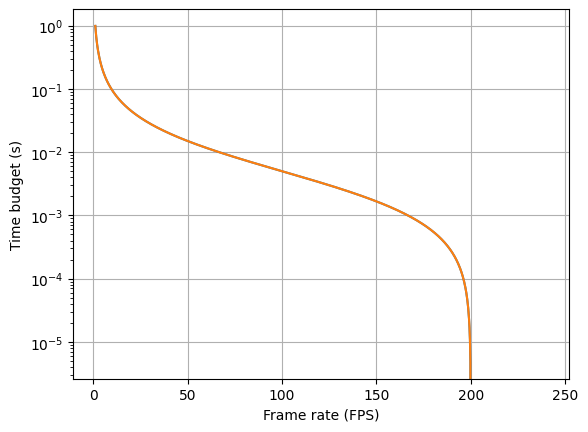
\includegraphics[width=0.5\linewidth]{assets/fps_vs_budget.png}
    \caption{An increase in frame rate lowers the maximum reconfiguration time budget}
    \label{fig:fps_vs_budget}
\end{figure}

\begin{table}[htbp]
\centering
\begin{tabular}{@{}lll@{}}
\toprule
Frame rate (FPS) & Frame time (ms) & Reconf. budget (ms) \\ \midrule
15               & 66.7            & 61.7                \\
24               & 41.7            & 36.7                \\
30               & 33.3            & 28.3                \\
60               & 16.7            & 11.7                \\
120              & 8.3             & 3.3                 \\
200              & 5               & 0                   \\
240              & 4.2             & -0.8                \\ \bottomrule
\end{tabular}
\caption{Reconfiguration time budget for different common video frame rates. The frame times and reconfiguration budgets are rounded.}
\label{tab:common_fps}
\end{table}

\Cref{tab:common_fps} shows a list of common video frame rates with their associated reconfiguration time budget.
A frame rate with zero or negative time budget means that the \graicore{} cannot be reconfigured seamlessly for a video with that frame rate.
Exceeding this time budget results into a delayed output which is undesirable since it negatively affects the user experience.
At a frame rate of $\SI{200}{FPS}$, the time budget is exactly zero, indicating that this represents the tight upper bound.
\Cref{fig:reconfig_time_line_ex} shows two time lines exemplifying a seamless and non-seamless reconfiguration procedure.

In terms of bandwidth, to reconfigure the \graicore{} fully (i.e., write all $\SI{36}{MB}$ of local memory), we require a minimum of $\SI{3086}{MB/s}$\footnote{$\frac{36}{\frac{1}{60} - 5 \times 10^{-3}} \approx 3086$} for $\SI{60}{FPS}$.
Note that this bandwidth number does not include any overhead induced by communication protocols. Therefore, in practice, the required minimum bandwidth is higher. 

With a technique such as layer-by-layer replacement, pipelining of configuration and processing can be achieved \cite{jiDemandLayeringRealTime2022}.
However, there are a multitude of challenges associated with this technique. 
Firstly, the sizes of an old (already processed) layer and a new (to be replaced with) layer may differ.
Replacing a layer is straightforward when the new layer is equal or smaller in size.
However, if the new layer is larger in size, it cannot fit as a whole.
It will need to replace multiple old layers to able to fit.
Secondly, the system will need a way to notify the relevant parties that a specific layer has completed processing.
This is required for indicating that a layer (or multiple layers) can be replaced by a new one. %synchronization
Finally, the time it takes to process a layer has not been explored before.
This is crucial to provide us a number that can be used to determine the reconfiguration time budget.
Due to these additional complexities, we have opted not to consider this technique.
Furthermore, we only consider the scenario where each frame is processed by a single model and reconfiguration may only happen whenever a frame has finished processing.

\begin{figure}[htbp]
    \centering
    \subfloat[]{
        \begin{tikzpicture}[scale=0.5]
    \draw[] (6,0) -- (24,0);
    \draw[dashed, ->] (24,0) -- (25,0);
    \draw (6,0.5) -- (6,-0.5) node[below] {$t_{0}$};
    \draw (12,0.5) -- (12,-0.5) node[below] {$t_{1}$};
    \draw (18,0.5) -- (18,-0.5) node[below] {$t_{2}$};
    \draw (24,0.5) -- (24,-0.5) node[below] {$t_{3}$};

    \draw [pattern=north east lines, pattern color=gray, line width = 1pt, very thick] ($(6,0)$) rectangle ++($(1.5,1)$) node[midway] {P};
    \draw [pattern=north west lines, pattern color=gray, line width = 1pt, very thick] ($(7.5,0)$) rectangle ++($(3,1)$) node[midway] {C};
    \draw [decorate,decoration={brace,amplitude=6pt}]($(6,1.5)$) -- ++($(1.5,0)$) node [black,midway,above=6pt] {\tiny L};
    
    \draw [pattern=north east lines, pattern color=gray, line width = 1pt, very thick] ($(12,0)$) rectangle ++($(1.5,1)$) node[midway] {P};
    \draw [pattern=north west lines, pattern color=gray, line width = 1pt, very thick] ($(13.5,0)$) rectangle ++($(3,1)$) node[midway] {C};
    \draw [decorate,decoration={brace,amplitude=6pt}]($(12,1.5)$) -- ++($(1.5,0)$) node [black,midway,above=6pt] {\tiny L};
    
    \draw [pattern=north west lines, pattern color=gray, line width = 1pt, very thick] ($(18,0)$) rectangle ++($(1.5,1)$) node[midway] {P};
    \draw [pattern=north west lines, pattern color=gray, line width = 1pt, very thick] ($(19.5,0)$) rectangle ++($(3,1)$) node[midway] {C};
    \draw [decorate,decoration={brace,amplitude=6pt}]($(18,1.5)$) -- ++($(1.5,0)$) node [black,midway,above=6pt] {\tiny L};
\end{tikzpicture}

        \label{fig:correct_reconfig}
    } \\
    \subfloat[]{
        \begin{tikzpicture}[scale=0.5]
    \draw[] (6,0) -- (24,0);
    \draw[dashed, ->] (24,0) -- (25,0);
    \draw (6,0.5) -- (6,-0.5) node[below] {$t_{0}$};
    \draw (12,0.5) -- (12,-0.5) node[below] {$t_{1}$};
    \draw (18,0.5) -- (18,-0.5) node[below] {$t_{2}$};
    \draw (24,0.5) -- (24,-0.5) node[below] {$t_{3}$};

    \draw [pattern=north east lines, pattern color=gray, line width = 1pt, very thick] ($(6,0)$) rectangle ++($(1.5,1)$) node[midway] {P};
    \draw [pattern=north west lines, pattern color=gray, line width = 1pt, very thick] ($(7.5,0)$) rectangle ++($(5,1)$) node[midway] {C};
    \draw [decorate,decoration={brace,amplitude=6pt}]($(6,1.5)$) -- ++($(1.5,0)$) node [black,midway,above=6pt] {\tiny L};
    
    \draw [pattern=north east lines, pattern color=gray, line width = 1pt, very thick] ($(12.5,0)$) rectangle ++($(1.5,1)$) node[midway] {P};
    \draw [pattern=north west lines, pattern color=gray, line width = 1pt, very thick] ($(14,0)$) rectangle ++($(5,1)$) node[midway] {C};
    \draw [decorate,decoration={brace,amplitude=6pt}]($(12,1.5)$) -- ++($(2,0)$) node [black,midway,above=6pt] {\tiny L};
    
    \draw [pattern=north west lines, pattern color=gray, line width = 1pt, very thick] ($(19,0)$) rectangle ++($(1.5,1)$) node[midway] {P};
    % \draw [pattern=north west lines, pattern color=gray, line width = 1pt, very thick] ($(20.5,0)$) rectangle ++($(5,1)$) node[midway] {C};
    \draw [decorate,decoration={brace,amplitude=6pt}]($(18,1.5)$) -- ++($(2.5,0)$) node [black,midway,above=6pt] {\tiny L};
    \node[right] at (20.5,0.5) {\ldots};



\end{tikzpicture}
        \label{fig:incorrect_reconfig}
    }
    \caption{
    Example time lines of reconfiguration procedures.
    $t_n$ indicates the time instance where the $n$th frame has been received by the \graicore{}, ready to be processed.
    At $t_0$, the \graicore{} is already configured with an initial model.
    In \protect\subref{fig:correct_reconfig}, the \graicore{} uses a different model for each consecutive frame.
    After receiving and processing (P) the very first frame at $t_0$, it starts reconfiguration (C) to a new model.
    Since the sum of the reconfiguration and processing time does not exceed the frame time ($t_{n+1} - t_{n})$, the frame processing latency (L) is equal for every incoming frame.
    The invariant latency is desired and indicates a seamless reconfiguration.
    \protect\subref{fig:incorrect_reconfig} has an increased reconfiguration time.
    Now, the sum of the reconfiguration and processing time does exceed the frame time.
    As a consequence, the frame processing latency increases for each incoming frame.
    In the long run, this latency will grow to infinity.
    Since the latency varies, this is an example of a non-seamless reconfiguration.
    }
    \label{fig:reconfig_time_line_ex}
\end{figure}

\subsubsection{Large model}

Due to the \graicore{} having limited memory capacity, a single large model cannot be loaded onto it at once.
Several works have proposed strategies for deploying CNNs on resource-constrained devices.
Among these strategies, "partitioning" refers to splitting an entire model at specific locations to create one or more partitions, thereby reducing instantaneous memory requirements \cite{kaboubiHybridPartitioningEmbedded2023}.
To fully process a frame, one or more (partial) reconfigurations will need to be performed.
Each of the reconfigurations will load in the subsequent neural network part needed for further processing.

For this case, a specific timing or bandwidth cannot be as easily determined.
This is due to the nature of a large model. A large model can be of any arbitrary size.
With a larger model having to be partitioned into more parts.
Consequently, an increase in parts sees an increase in the amount of reconfigurations necessary to execute the large model completely.
Due to this, determining the total reconfiguration time budget is more involved.
A single frame is ``processed'' multiple times, once by each part of the neural network.
The total reconfiguration time budget is dependent on the number of (partial) reconfigurations necessary to fully process a single frame.

\begin{table}[hbtp]
\centering
\begin{tabular}{@{}lllllll@{}}
\toprule
    &            & \multicolumn{5}{l}{Time budget per reconfiguration amount (ms)} \\
FPS & Frame time (ms) & 1x         & 2x          & 3x         & 4x         & 5x         \\ \midrule
5   & 200  & 195  & 190  & 185  & 180   & 175   \\
15  & 66.7 & 61.7 & 56.7 & 51.7 & 46.7  & 41.7  \\
24  & 41.7 & 36.7 & 31.7 & 26.7 & 21.7  & 16.7  \\
30  & 33.3 & 28.3 & 23.3 & 18.3 & 13.3  & 8.3   \\
60  & 16.7 & 11.7 & 6.7  & 1.7  & -3.3  & -8.3  \\
120 & 8.3  & 3.3  & -1.7 & -6.7 & -11.7 & -16.7 \\ \bottomrule
\end{tabular}
\caption{Maximum reconfiguration time budget for common frame rates and different reconfiguration amounts. The frame times and time budgets are rounded.}
\label{tab:common_fps_reconfig_amount}
\end{table}

As an example, assume that a large model is partitioned into an arbitrary amount of parts.
Each part is exactly the size of the \graicore{}'s total capacity and the processing time for each part takes $\SI{5}{ms}$.
\Cref{tab:common_fps_reconfig_amount} shows that for a video of $\SI{60}{FPS}$ and a large model requiring two reconfigurations, we have a maximum reconfiguration time budget of $\SI{6.7}{ms}$.
Notice that a large model that requires $4$ reconfigurations at \SI{60}{FPS} has a negative time budget.
This means that it is not possible to process a frame for a video of \SI{60}{FPS} within two consecutive incoming frames for that particular model.
Processing frames at \SI{60}{FPS} with a large model is often not feasible, as many models require more than a few reconfigurations.
A lower frame rate gives us a larger reconfiguration budget, which is more suitable for larger models.
Notably, reducing the frame rate to single digits significantly increases the available reconfiguration budget.
\Cref{fig:larger_reconfig_ex} illustrates two time lines showing a good and a bad scenario.

\begin{figure}[htbp]
    \centering
    \subfloat[]{
        \begin{tikzpicture}[scale=0.5]

    \draw[] (6,0) -- (24,0);
    % \draw[dashed, <-] (5,0) -- (6,0);
    \draw[dashed, ->] (24,0) -- (25,0);
    \draw (6,0.5) -- (6,-0.5) node[below] {$t_{0}$};
    \draw (12,0.5) -- (12,-0.5) node[below] {$t_{1}$};
    \draw (18,0.5) -- (18,-0.5) node[below] {$t_{2}$};
    \draw (24,0.5) -- (24,-0.5) node[below] {$t_{3}$};
    
    \draw [pattern=north east lines, pattern color=gray, line width = 1pt, very thick] ($(6,0)$) rectangle ++($(1,1)$) node[midway] {P};
    \draw [pattern=north west lines, pattern color=gray, line width = 1pt, very thick] ($(7,0)$) rectangle ++($(1.5,1)$) node[midway] {C};
    \draw [pattern=north east lines, pattern color=gray, line width = 1pt, very thick] ($(8.5,0)$) rectangle ++($(1,1)$) node[midway] {P};
    \draw [pattern=north west lines, pattern color=gray, line width = 1pt, very thick] ($(9.5,0)$) rectangle ++($(1.5,1)$) node[midway] {C};
    \draw [decorate,decoration={brace,amplitude=6pt}]($(6,1.5)$) -- ++($(3.5,0)$) node [black,midway,above=6pt] {\tiny L};
    
    \draw [pattern=north east lines, pattern color=gray, line width = 1pt, very thick] ($(12,0)$) rectangle ++($(1,1)$) node[midway] {P};
    \draw [pattern=north west lines, pattern color=gray, line width = 1pt, very thick] ($(13,0)$) rectangle ++($(1.5,1)$) node[midway] {C};
    \draw [pattern=north east lines, pattern color=gray, line width = 1pt, very thick] ($(14.5,0)$) rectangle ++($(1,1)$) node[midway] {P};
    \draw [pattern=north west lines, pattern color=gray, line width = 1pt, very thick] ($(15.5,0)$) rectangle ++($(1.5,1)$) node[midway] {C};
    \draw [decorate,decoration={brace,amplitude=6pt}]($(12,1.5)$) -- ++($(3.5,0)$) node [black,midway,above=6pt] {\tiny L};
    
    \draw [pattern=north east lines, pattern color=gray, line width = 1pt, very thick] ($(18,0)$) rectangle ++($(1,1)$) node[midway] {P};
    \draw [pattern=north west lines, pattern color=gray, line width = 1pt, very thick] ($(19,0)$) rectangle ++($(1.5,1)$) node[midway] {C};
    \draw [pattern=north east lines, pattern color=gray, line width = 1pt, very thick] ($(20.5,0)$) rectangle ++($(1,1)$) node[midway] {P};
    \draw [pattern=north west lines, pattern color=gray, line width = 1pt, very thick] ($(21.5,0)$) rectangle ++($(1.5,1)$) node[midway] {C};
    \draw [decorate,decoration={brace,amplitude=6pt}]($(18,1.5)$) -- ++($(3.5,0)$) node [black,midway,above=6pt] {\tiny L};
\end{tikzpicture}

        \label{fig:large_reconfig_ex1}
    } \\
    \subfloat[]{
        \begin{tikzpicture}[scale=0.5]

    \draw[] (6,0) -- (24,0);
    \draw[dashed, ->] (24,0) -- (25,0);
    \draw (6,0.5) -- (6,-0.5) node[below] {$t_{0}$};
    \draw (12,0.5) -- (12,-0.5) node[below] {$t_{1}$};
    \draw (18,0.5) -- (18,-0.5) node[below] {$t_{2}$};
    \draw (24,0.5) -- (24,-0.5) node[below] {$t_{3}$};
    
    \draw [pattern=north east lines, pattern color=gray, line width = 1pt, very thick] ($(6,0)$) rectangle ++($(1,1)$) node[midway] {P};
    \draw [pattern=north west lines, pattern color=gray, line width = 1pt, very thick] ($(7,0)$) rectangle ++($(2.25,1)$) node[midway] {C};
    \draw [pattern=north east lines, pattern color=gray, line width = 1pt, very thick] ($(9.25,0)$) rectangle ++($(1,1)$) node[midway] {P};
    \draw [pattern=north west lines, pattern color=gray, line width = 1pt, very thick] ($(10.25,0)$) rectangle ++($(2.25,1)$) node[midway] {C};
    \draw [decorate,decoration={brace,amplitude=6pt}]($(6,1.5)$) -- ++($(4.25,0)$) node [black,midway,above=6pt] {\tiny L};
    
    \draw [pattern=north east lines, pattern color=gray, line width = 1pt, very thick] ($(12.5,0)$) rectangle ++($(1,1)$) node[midway] {P};
    \draw [pattern=north west lines, pattern color=gray, line width = 1pt, very thick] ($(13.5,0)$) rectangle ++($(2.25,1)$) node[midway] {C};
    \draw [pattern=north east lines, pattern color=gray, line width = 1pt, very thick] ($(15.75,0)$) rectangle ++($(1,1)$) node[midway] {P};
    \draw [pattern=north west lines, pattern color=gray, line width = 1pt, very thick] ($(16.75,0)$) rectangle ++($(2.25,1)$) node[midway] {C};
    \draw [decorate,decoration={brace,amplitude=6pt}]($(12,1.5)$) -- ++($(4.75,0)$) node [black,midway,above=6pt] {\tiny L};
    
    \draw [pattern=north east lines, pattern color=gray, line width = 1pt, very thick] ($(19,0)$) rectangle ++($(1,1)$) node[midway] {P};
    \draw [pattern=north west lines, pattern color=gray, line width = 1pt, very thick] ($(20,0)$) rectangle ++($(2.25,1)$) node[midway] {C};
    \draw [pattern=north east lines, pattern color=gray, line width = 1pt, very thick] ($(22.25,0)$) rectangle ++($(1,1)$) node[midway] {P};
    % \draw [pattern=north west lines, pattern color=gray, line width = 1pt, very thick] ($(23.25,0)$) rectangle ++($(2.25,1)$) node[midway] {C};
    \node[right] at (23.25,0.5) {\ldots};
    \draw [decorate,decoration={brace,amplitude=6pt}]($(18,1.5)$) -- ++($(5.25,0)$) node [black,midway,above=6pt] {\tiny L};

\end{tikzpicture}
        \label{fig:large_reconfig_ex2}
    }
    \caption{
        Example time lines of processing a large model requiring two reconfigurations.
        At $t_0$, the \graicore{} is already configured with the first part of the model.
        In \protect\subref{fig:large_reconfig_ex1}, the two reconfiguration periods (C) and two processing periods (P) fit within the reception of two consecutive frames ($t_n$ and $t_{n+1}$).
        The frame processing latency (L) is equal for every incoming frame.
        In \protect\subref{fig:large_reconfig_ex2}, the reconfiguration time is increased. 
        This results into an ever-increasing frame processing latency.
    }
    \label{fig:larger_reconfig_ex}
\end{figure}

We will examine realistic AI models, specifically the ResNet-101 model \cite{heDeepResidualLearning2015}, which is a potential use case for the \graicore{} and exceeds its local memory, to understand the required timings and bandwidth.
This analysis will provide insights into the bandwidth requirements and power usage of a large AI model.
However, given the complexity of this analysis, it will be deferred to the project phase.

\subsubsection{Power consumption}
Since the \graicore{} is primarily used as an AI accelerator for edge devices, maintaining low power consumption is crucial.
The addition of external memory with the capability to reconfigure the \graicore{} will inevitably increase the overall power consumption of the system.
However, specific optimizations can be implemented to minimize this increase.
The solution should encompass the memory, interface, and controller, with a focus on achieving minimal power usage.

We are considering options such as DRAM or NVM, and the final selection will balance power efficiency, performance, and system compatibility.
It has been measured that the \graicore{} consumes between \SI{200}{mW} and \SI{500}{mW} when processing frames at \SI{60}{FPS}.
We aim to not exceed \SI{20}{mW} when performing 60 reconfigurations per second.
